\begin{savequote}[8cm]
It's simple mathematics.
  \qauthor{--- Mos Def, "Mathematics"}
\end{savequote}

\chapter{\label{ch:3-methods}Theory and Methodology}

\minitoc

%% Books:

% For a really nice explanation of solid state QM basics - bloch waves, an electron in a crystal potential etc, see Lundstrom "fundamentals of carrier transport"

\section{Introduction} 

In this chapter I present the theory and methodology that underlies the work in this thesis. The chapter starts with an introduction to Density Functional Theory - first I introduce the theoretical concepts, then I provide details about how DFT is implemented in practice. In the second part of the chapter I outline how we can use DFT energies combined with a number of post-processing steps to predict defect formation energies and charge transition levels. The chapter ends with an introduction to the theory of lattice dynamics and how this is used to calculate the vibrational properties of a material. 

\section{Density Functional Theory} \label{DFTtheory}

Density Functional Theory is the most commonly used method of electronic structure calculation in condensed matter physics and quantum chemistry. 
Using DFT we are able to predict the ground state properties of a material including electron density, total energy, equilibrium structure, vibrational frequencies and properties relating to the difference in total energies, such as defect formation energies or surface energies. 
As DFT is a ground state theory, we are not able to calculate properties relating to to excited states and, without further calculations (such as those outlined in Section \ref{sec:latticedynamics}), results do not incorporate the effects of temperature. 

The theoretical basis for DFT was established in 1964 through the work of Walter Kohn and Pierre Hohenberg.\autocite{Hohenberg1964} This was further developed by Walter Kohn and Lu Jeu Sham to produce Kohn-Sham DFT.\autocite{Kohn1965} However it was not until the late 1980's that work started on building approximations to the exchange-correlation functional so that DFT could be used in practice. 

There are a growing number of codes that implement DFT, many of which include extensions to DFT so that excited state properties can be predicted.
Although some codes aspire to a blackbox approach, with the user protected from the underlying mechanics of DFT, for most systems of interest an understanding of the underlying approximations and parameters used are required for reliable results.

\subsection{DFT in theory} %expand to include more equations, including slater determinant? and E\phi=H\phi.

Firstly, a note on the name. A function accepts one or more numbers as input and produces a number as output. Likewise, a functional accepts one or more \textit{functions} as inputs, and produces a number as output. In DFT the functional is the electron density which is a function of space and time.

Throughout this chapter, unless stated otherwise, we use the Born-Oppenheimer approximation: the heavy atomic nuclei are treated as fixed points, and we solve the ground state quantum mechanical problem for the electrons only. This reduces the number of degrees of freedom of the system, a tactic that will be used again later in the chapter.

Although no one single text is followed, concepts for the underlying theory have been taken from References \cite{Burke2007}, \cite{Scuseria05} and \cite{Perdew2010}.


\subsubsection{The Schr\"{o}dinger equation}

The Schr\"{o}dinger equation describes the wavefunction $\Psi$ of a quantum mechanical system. The wavefunction is a fundamental postulate of quantum mechanics and it contains all the information for a given system. Once the Schr\"{o}dinger equation is solved, and a wavefunction is found, all the physical properties for that system follow. To take the simplest possible example, the time-independent non-relativistic Schr\"{o}dinger equation for a single particle can be written as:
\begin{equation}
\left[\frac{-\hbar^2}{2m}\nabla^2+V(\textbf{r})\right]\Psi(\textbf{r}) = E\Psi(\textbf{r})
\end{equation}
where the first term in the bracket corresponds to the kinetic energy and the second term corresponds to the potential energy. For a single particle in a simple potential, such as the ``particle in a box" system or hydrogen atom, the Schr\"{o}dinger equation can be solved exactly. Unfortunately it is not possible to solve the Schr\"{o}dinger equation exactly for more complex systems, where there are multiple electrons interacting with each other (N-body or many-body systems). In this case, the Schr\"{o}dinger equation takes the form:
\begin{equation}
\left[\frac{-\hbar^2}{2m}\sum_{i=1}^N\nabla_i^2+\sum_{i=1}^Nv_{\textrm{ext}}(\textbf{r}_i)+\sum_{i<j}^N\frac{q_iq_j}{\lvert\textbf{r}_i-\textbf{r}_j\rvert}\right]\Psi(\textbf{r}_i) = E\Psi(\textbf{r}_i),
\end{equation}
where the third term in the square bracket describes the electrostatic interaction between two particles of charges $q_i$ and $q_j$, and couples the coordinates of the particles together.

The following methods (Hartree-Fock and Kohn-Sham DFT) give a way to obtain an approximate solution to the Schr\"{o}dinger equation for systems of interest. They do this by mapping the interacting problem onto a non-interacting problem with an effective potential $V_\textrm{s}(\textbf{r})$. In doing so, the dimensionality of the problem is greatly reduced. Instead of solving one N-dimensional probelem, which is computationally intractable, N one-dimensional problems are solved (Figure \ref{decouple}). These provide a compromise between accuracy and computational efficiency.

\begin{figure}[h]
\centering
  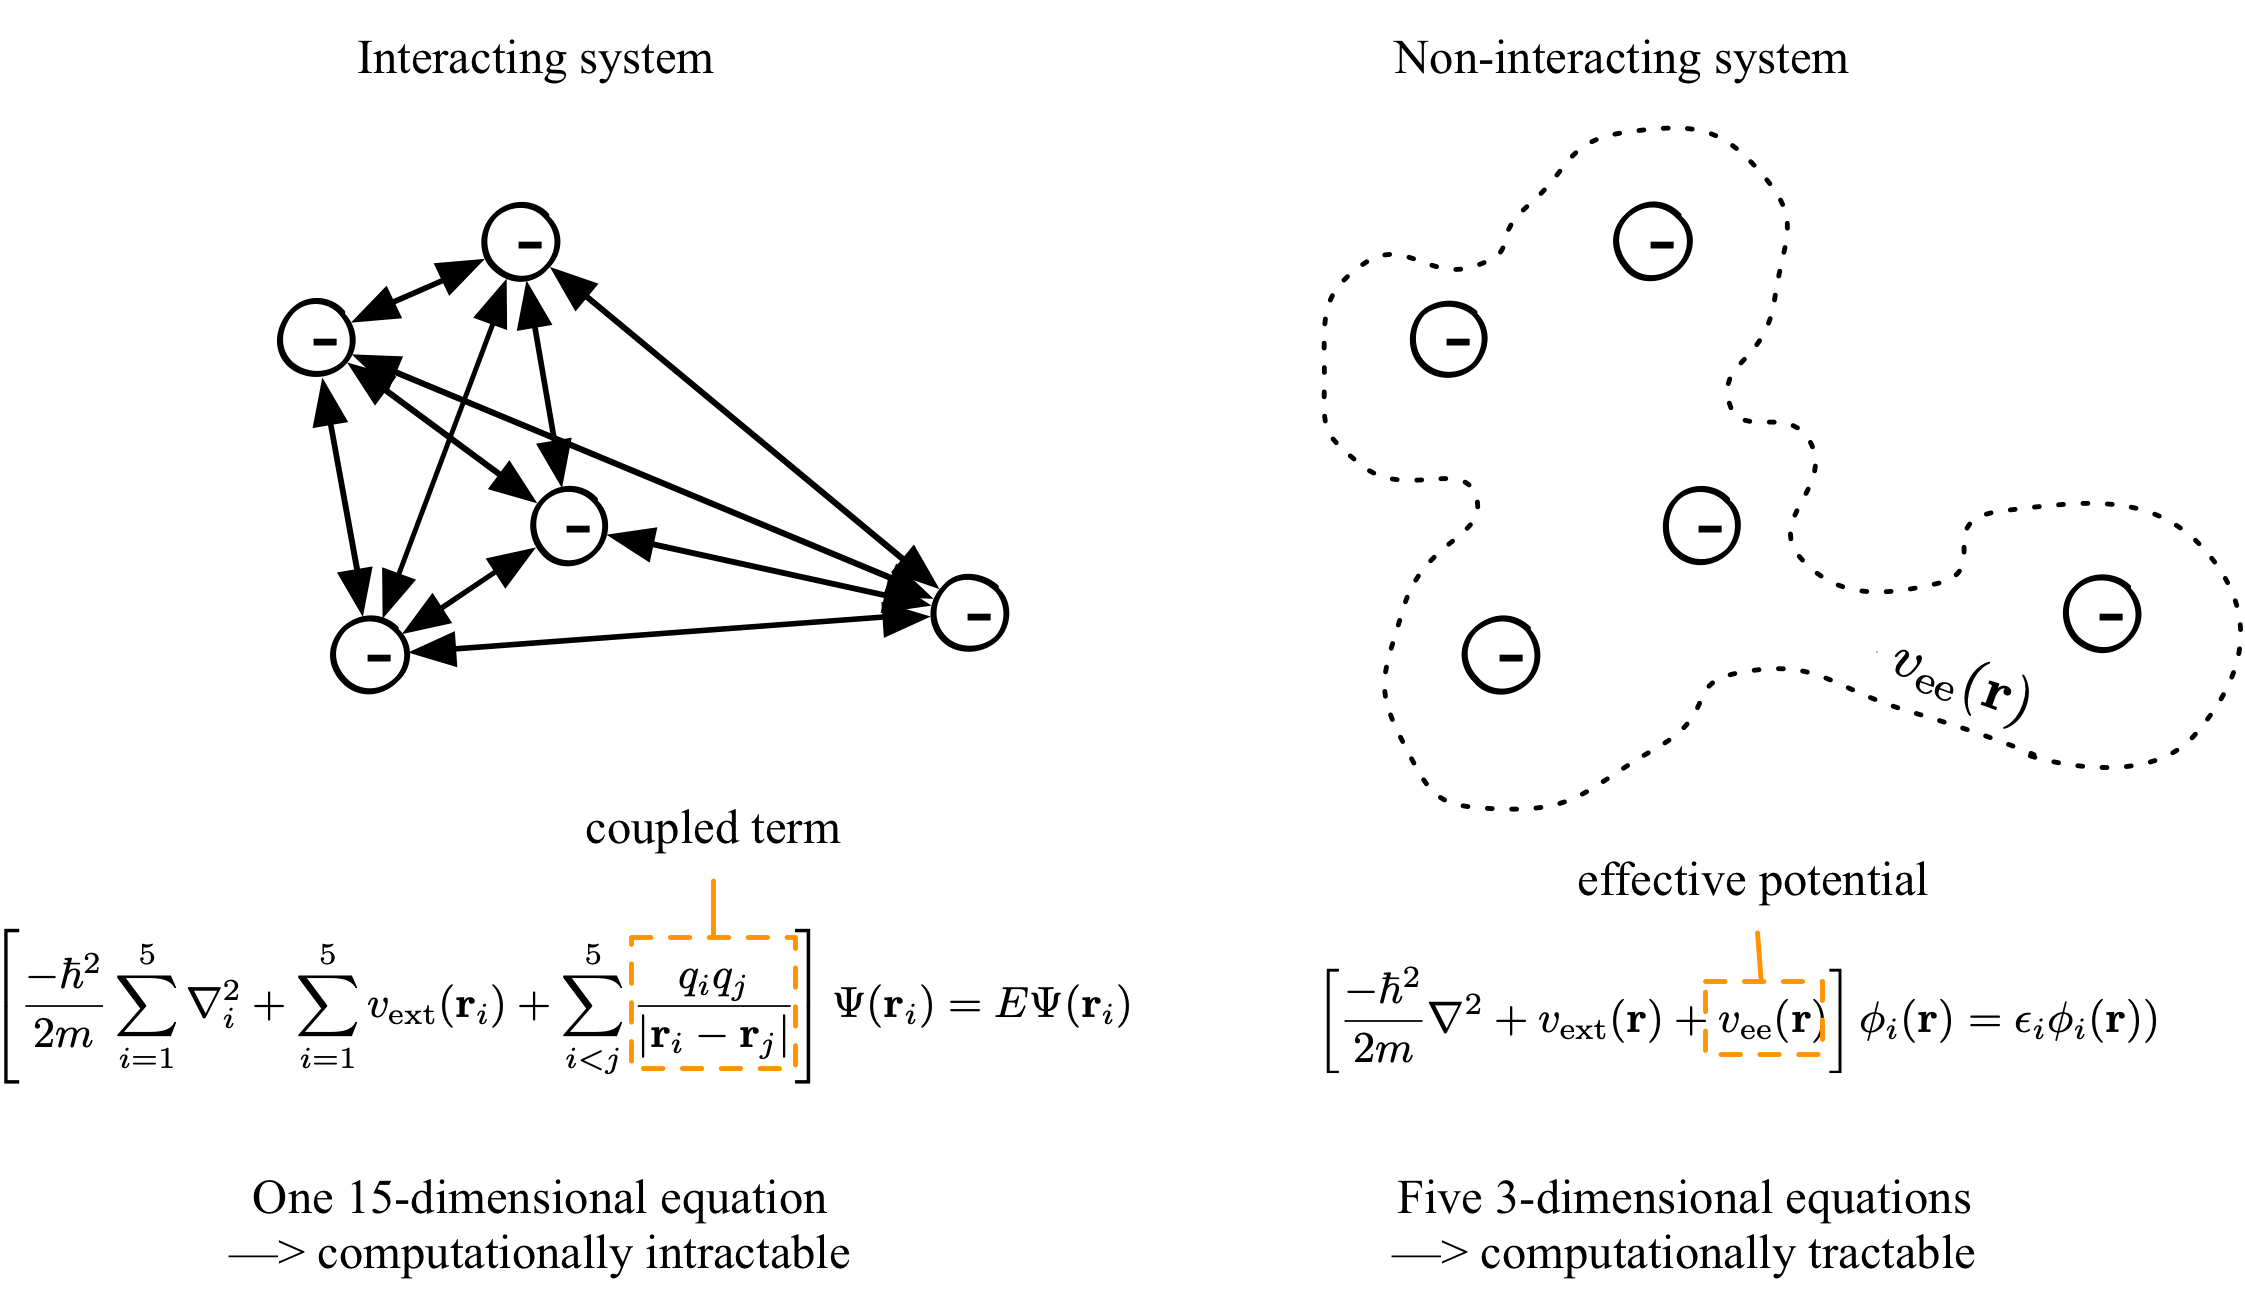
\includegraphics[width=1.0\columnwidth]{figures/ch3/decouple.png}
  \caption[Schematic outlining the equivalence between interacting and non-interacting systems]{Schematic outlining the equivalence between a system of interacting particles and a system of non-interacting particles in an effective potential. The underlying idea is that an interaction can be replaced by the equivalent potential. This maps the interacting 3N-dimensional problem onto N 3-dimensional problems. A consequence of this mapping is that the effective potential depends on the electron density which is itself dependant on the effective potential - a self-consistent set of equations is formed.} %update so q1q2 in couple term in picture
  \label{decouple}
\end{figure}

\subsubsection{Hartree-Fock methods}

Hartree-Fock methods introduced the concept of fictitious one-electron orbitals $\phi$ that do not interact with each other as a way of solving the Schr\"{o}dinger equation. The HF many-body wavefunction is a Slater determinant of the one-electron orbitals and is denoted with $\Phi$. 

The effective potential, introduced in Figure \ref{decouple}, is given by $V_{\textrm{ee}} = U + E_{\textrm{x}}$. $U$ accounts for the electrostatic interaction between electrons. Hartree-Fock methods model the charge interaction as a coulomb potential for a system of fixed electrons; the electrons feel the average electrostatic field due to the other electrons.

The second way electrons interact with each other is via their spin:
\begin{displayquote}
    Two MCs can't occupy the same space at the same time,
    it's against the laws of physics \\ \hspace{2cm}---Lauryn Hill, \textit{Zealots}
\end{displayquote}
Electrons with the same spin are indistinguishable, and a consequence of this is that the many body  wavefunction must be anti-symmetric. This leads to the Pauli Exclusion Principle, whereby two identical electrons (ie, electrons with the same spin and momentum) cannot occupy the same space at the same time. Hartree Fock methods account for electron exchange, the repulsion between electrons with parallel spins, exactly. 

Hartree-Fock methods do not give an exact solution to the Schr\"{o}dinger equation as they ignore electron correlation. This is the correlated motion of electrons with anti-parallel spins as a result of their mutual coulombic repulsion. It is a consequence of the fact that the true many body wavefunction is not formed from a simple Slater determinant.
% from http://newton.ex.ac.uk/research/qsystems/people/coomer/dft_intro.html

\subsubsection{The Hohenberg-Kohn theorems}

The 1964 Hohenberg-Kohn paper contains two key results: (i) the ground state electron density uniquely determines the ground state electronic wave function and, following this, all properties of the system; (ii) the true density functional for the electronic energy assumes its minimum for the correct ground-state density. % quote this from? http://publish.uwo.ca/~vstarove/PDF/tacc_chapter24.pdf

In Hartree-Fock methods, the potentials (external, coulomb and exchange) determine the properties of a system. First, Hohenberg and Kohn demonstrate that the density can be used instead to uniquely characterise the system; rather than solving the Schr\"{o}dinger equation for the wavefunction, we can solve it for the electron density. The energy can be expressed as
$$E\left[\rho\right]=\int v_{\textrm{ext}}(\textbf{r})\rho(\textbf{r})d\textbf{r}+T\left[\rho\right]+J\left[\rho\right]+E_{\textrm{xc}}\left[\rho\right].$$
For a fixed number of electrons the functional $F\left[\rho\right]=T\left[\rho\right]+J\left[\rho\right]+E_{\textrm{xc}}\left[\rho\right]$ is universal, and the only thing that varies between systems is the external potential (determined by the electron-nuclei interaction). 

Secondly, Hohenberg and Kohn show that the ground state energy can be found variationally; the density that minimises the total energy is the true ground state density.

This formalism has the advantage that the electron density has a lower dimensionality than the N-electron wavefunction (Figure \ref{}). The problem is that although the Hohenberg-Kohn theorem tells us that the terms $T\left[\rho\right]$ and $E_{\textrm{xc}}\left[\rho\right]$ exist, they are unknown and must be approximated.

\begin{figure}[h]
\centering
  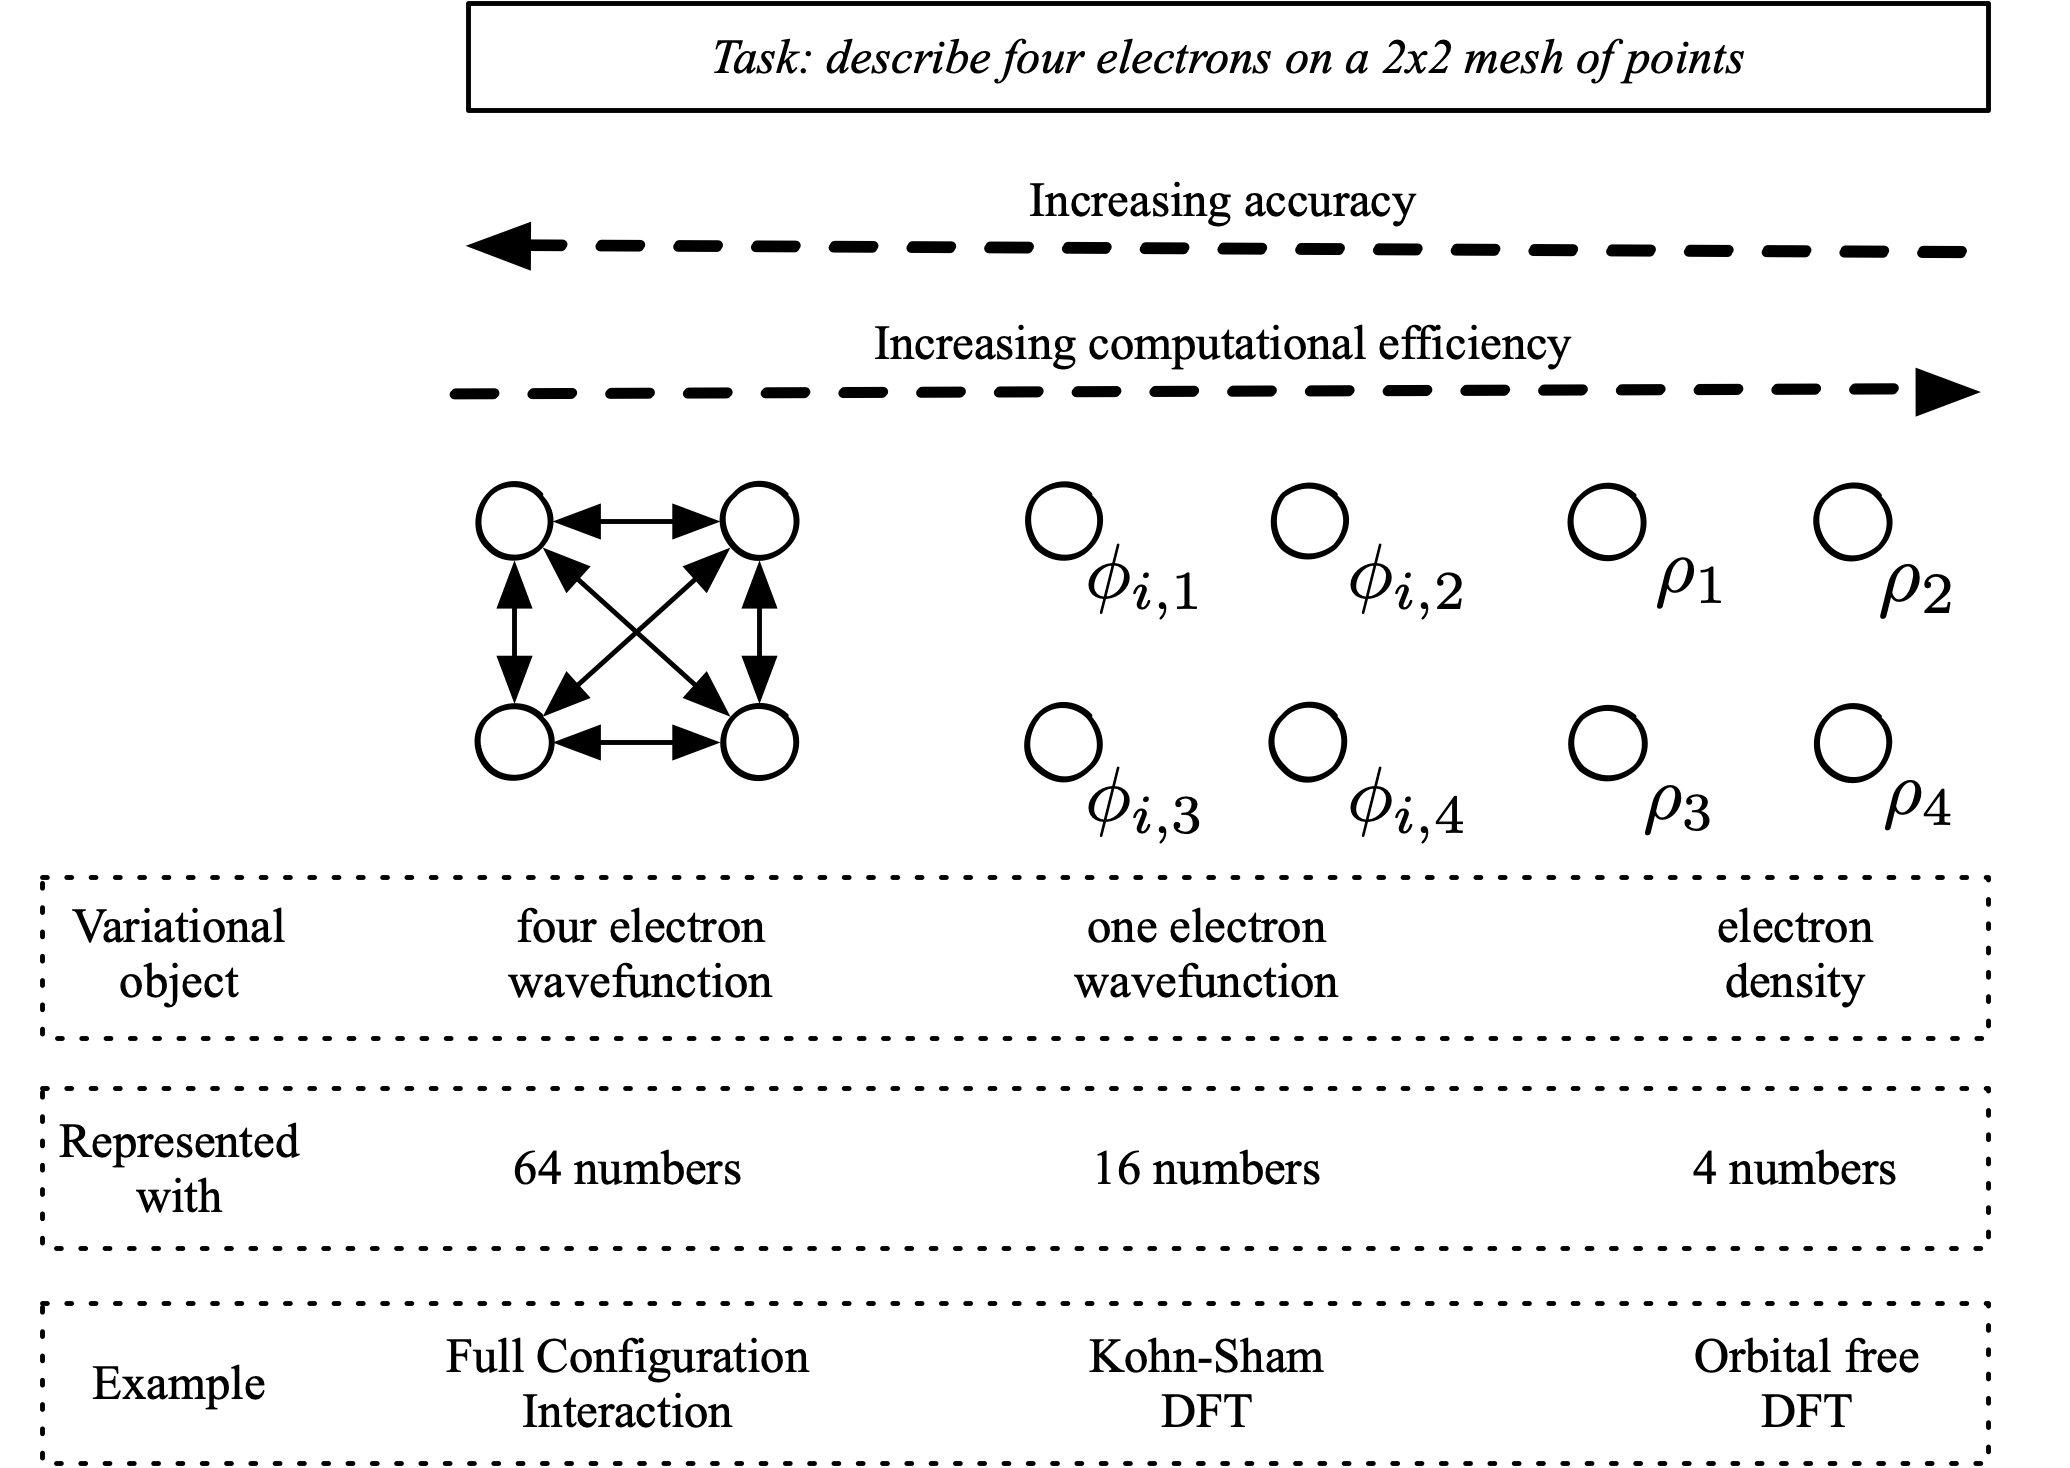
\includegraphics[width=1.0\columnwidth]{figures/ch3/dimensions.png}
  \caption[Dimensionality of variational objects]{To solve the Schr\"{o}dinger equation we can use a variational object with lower dimensionality and higher computational efficiency, although this will come at the cost of accuracy. This schematic is based on a discussion in Walter Kohn's Nobel Prize lecture.\autocite{Kohn1999}}
  \label{decouple}
\end{figure}
% Is this right? I don't understand how the two electron wavefunction scales (4^2) - it's discussed in the 14 easy lessons.


\subsubsection{The Kohn-Sham theorem} 

The Kohn-Sham theorem shows the for any interacting system with ground state density $\rho(\textrm{r})$ there exists a non-interacting system with the same ground-state $\rho(\textrm{r})$. To find the ground state energy of the real interacting system, the occupation numbers of \textit{fictitous}, non-interacting one-electron orbitals can be optimised. For a non-interacting system we know how to calculate $T\left[\rho\right]$ and this provides a good approximation to the true kinetic energy, so the Kohn-Sham theorem provide a more practical way to apply DFT. However, the exchange-correlation density functional $E_{\textrm{xc}}\left[\rho\right]$ is still not known. Only approximations to this functional can be made, leading to approximations for the electronic density, total energy and other system properties.


\subsection{DFT in practice}

\subsubsection{Exchange-correlation functionals}
To use Kohn-Sham DFT we must approximate the exchange-correlation functional, and there is a growing list of functionals with varying levels of complexity. A useful way of categorising these functionals, "Jacob's Ladder", has been proposed by John Perdew (Figure \ref{}). As a general rule, more accurate functionals are constructured by adding more parameters and variables.

\begin{figure}[h]
\centering
  \includegraphics[width=1.0\columnwidth]{figures/ch3/jacobsladder.png}
  \caption[Jacob's ladder of exchange-correlation functionals]{}
  \label{decouple}
\end{figure}

\textit{Local Density Approximation} \\
At the lowest rung of the ladder is the local density approximation. In this approximation, only one variable is used to calculate the exchange correlation energy. This is the charge density for an infinitesimal 3-dimensional volume element. The exchange energy is calculated exactly
$$
E_{\textrm{LDA,x}}\left[n\right] = −\frac{3}{4}\left(\frac{3}{\pi}\right)^{\frac{1}{3}}n^{\frac{4}{3}}\left(\textbf{r}\right)d\textbf{r},
$$
and the correlation energy is calculated numerically by fitting to many-body quantum monte carlo studies for an inhomogeneous electron gas.%Ceperley and Alder
Strictly, the LDA should only be used for slowly varying densities, however it has performed surprisingly well for predicting the properties of a variety of atoms, solids and molecules. This is due to a cancellation of errors: LDA underestimates the exchange energy and overestimates the correlation energy. However there is a tendency for LDA to overestimate the binding energy and underestimate lattice parameters. This is a particularly pronounced problem in weakly bonded systems. Common LDA functionals include VWN and PW92.

\textit{Generalised Gradient Approximation} \\
At the next level of theory, two variables are used to determine the exchange-correlation energy: charge density and the density gradient. GGAs are semi-local functions due to their dependence on the gradient. The parameters of GGA functionals can be derived from physical constraints (non-empirical, as in the widely used PBE functional), or obtained from fitting procedures (empirical, as in the case of B88). GGAs improve the over-binding of LDA, but tend to underestimate the band gap of the material.

\textit{Meta-GGA} \\
Meta-GGAs extend the GGA functional to include the non-interacting kinetic energy density as an input to the functional. This is the calculated from the laplacian of the occupied electron orbitals.
% could include equation here perhaps (make sure consisstent with earlier).
A common meta-GGA functional is TPSS.

\textit{Hybrid functionals} \\
On the fourth rung, hybrid functionals combine GGA functionals with a proportion of the exact HF exchange energy. The simplest hybrid functional takes the form
$$
E_{\textrm{hybrid,xc}}\left[n\right] = \alpha E_{\textrm{exact,x}} + \left(1-\alpha\right)E_{\textrm{GGA,xc}}
$$
In some studies, the proportion of exact exchange is tuned to reproduce the property of interest correctly. For example, $\alpha=0.25$ is commonly used to correctly reproduce the band gap of the hybrid halide perovskite MAPI.% check the alpha is right
In DFT each electron interacts with itself as the potential derives from the total charge density of the system. This error is particularly pronounced for localised states, for example after the trapping of an electron or hole. By including a proportion of exact HF exchange hybrid functionals correct the self-interaction error and improve the accuracy of predictions.
% good stuff here incl. schematic: https://www.ncbi.nlm.nih.gov/pmc/articles/PMC4892865/#S3title
% - Linked to Koopman’s linearity:E(N) – E(N-1) = En
% See Janak 1978. 

\textit{Random Phase Approximation} \\
Closest to heaven is the Random Phase Approximation, which uses all of the Kohn-Sham orbitals (occupied and unoccupied) as input. Previous approaches fail when there are significant long range effects, as they have no information about the electron density far from an electron. The RPA is able to correctly predict long-range interactions between non-overlapping electron orbitals, for example van der Waals interactions.

% can I find plot of total energy as function of seperation using different approaches??
%As DFT is exact except for the approximation to the exchange-correlation functional, any shortcoming to a DFT prediction can be attributed to the XC-functional. It should be noted though that DFT 
% DFT was not designed to calculate band gaps.
% - However, since 2000 functionals have been better at giving total energy but they don’t give accurate density: straying away from ab-initio into a fitting exercise: DFT is straying from the path towards an exact functional

\subsubsection{Symmetry}

The material studied in this thesis, \ce{CH3NH3PbI3}, is a crystalline solid. Although we want to understand the properties of a finite piece of material, we use the standard approach which is to model the finite crystal as an infinite crystal. This is acceptable if the crystal piece is large enough so that it's properties do not depend on size. We introduce Born-von Karman (periodic) boundary conditions so that the infinite crystal is built from a repeating array of unit cells. For a unit cell of length $L$, any physically significant function $\psi$ of the crystal must have the same value at the origin and $L$, or in 3D:

$$ 
\psi([0 0 0]) = \psi([L 0 0]) =  \psi([ 0 L 0]) = \psi([0 0 L])
$$

where the square bracket denotes a vector on the basis of the three unit cell vectors (Figure \ref{translational}. Note that there are an infinite number of unit cells of different shapes and sizes that can be used to build an infinite crystal.

It is often the case that translational symmetry is broken in the real material, for example when there are point defects (as in Results chapter \ref{}). Furthermore, lattice vibrations have a periodicity larger than the unit cell (Results chapter \ref{}). To model this phenomena a supercell is built from multiple unit cells and this is used as the basic repeating unit (Figure \ref{translational}).

\begin{figure}[h]
\centering
  \includegraphics[width=1.0\columnwidth]{figures/ch3/translational.png}
  \caption[]{} 
  \label{translational}
\end{figure}


When the Schrodinger equation is solved for a H atom the solution gives wavefunctions corresponding to the 1s, 2s, 2p, etc orbitals found in chemistry. For periodic systems, wavefunctions are formed by Bl\:{o}ch functions:\autocite{Hoffman1987}

$$
\psi_nk(\textbf{r}) = u_k(\textbf{r})e^{i\textbf{k}\cdot\textbf{r}}
$$

where the Bl\:{o}ch function is formed from the product of a function $u_k$ with the same periodicity as the crystal lattice, and a plane wave $e^{i\textbf{k}\cdot\textbf{r}}$. $k$ is a crystal wave vector; to understand the physical significance of $k$ we consider an infinite 1D chain of hydrogen atoms separated at distance $L$. The electron states can be described a linear combination of H 1s orbitals $u_k$ centred at each lattice point :

$$
\psi_k = \sum_nu_ne^{iknL}
$$

$k=0$ corresponds to the most bonding state, and $k=\frac{\pi}{L}$ corresponds to the anti-bonding state
\begin{align}
\psi_0 &= \sum_nu_ne^0 = u_1 +u_2 +u_3 +u_4 \dots \\
\psi_{\frac{\pi}{L}} &= \sum_nu_ne^{i\pi n} = u_1 -u_2+u_3-u_4 \dots
\end{align}

Between these two extremes there is a continuum of states forming an electronic band (Figure \ref{bands}). The cystal vector $k$ fully determines the energy and so the energy can be plotted as a function of the $k$ vector. The $k$ vector forms a space known as reciprocal space. As a result of crystal symmetry, only $k$-vectors within a region of space known as the Brillouin Zone ($|k|<\frac{\pi}{a}$) need to be considered.

\begin{figure}[h]
\centering
  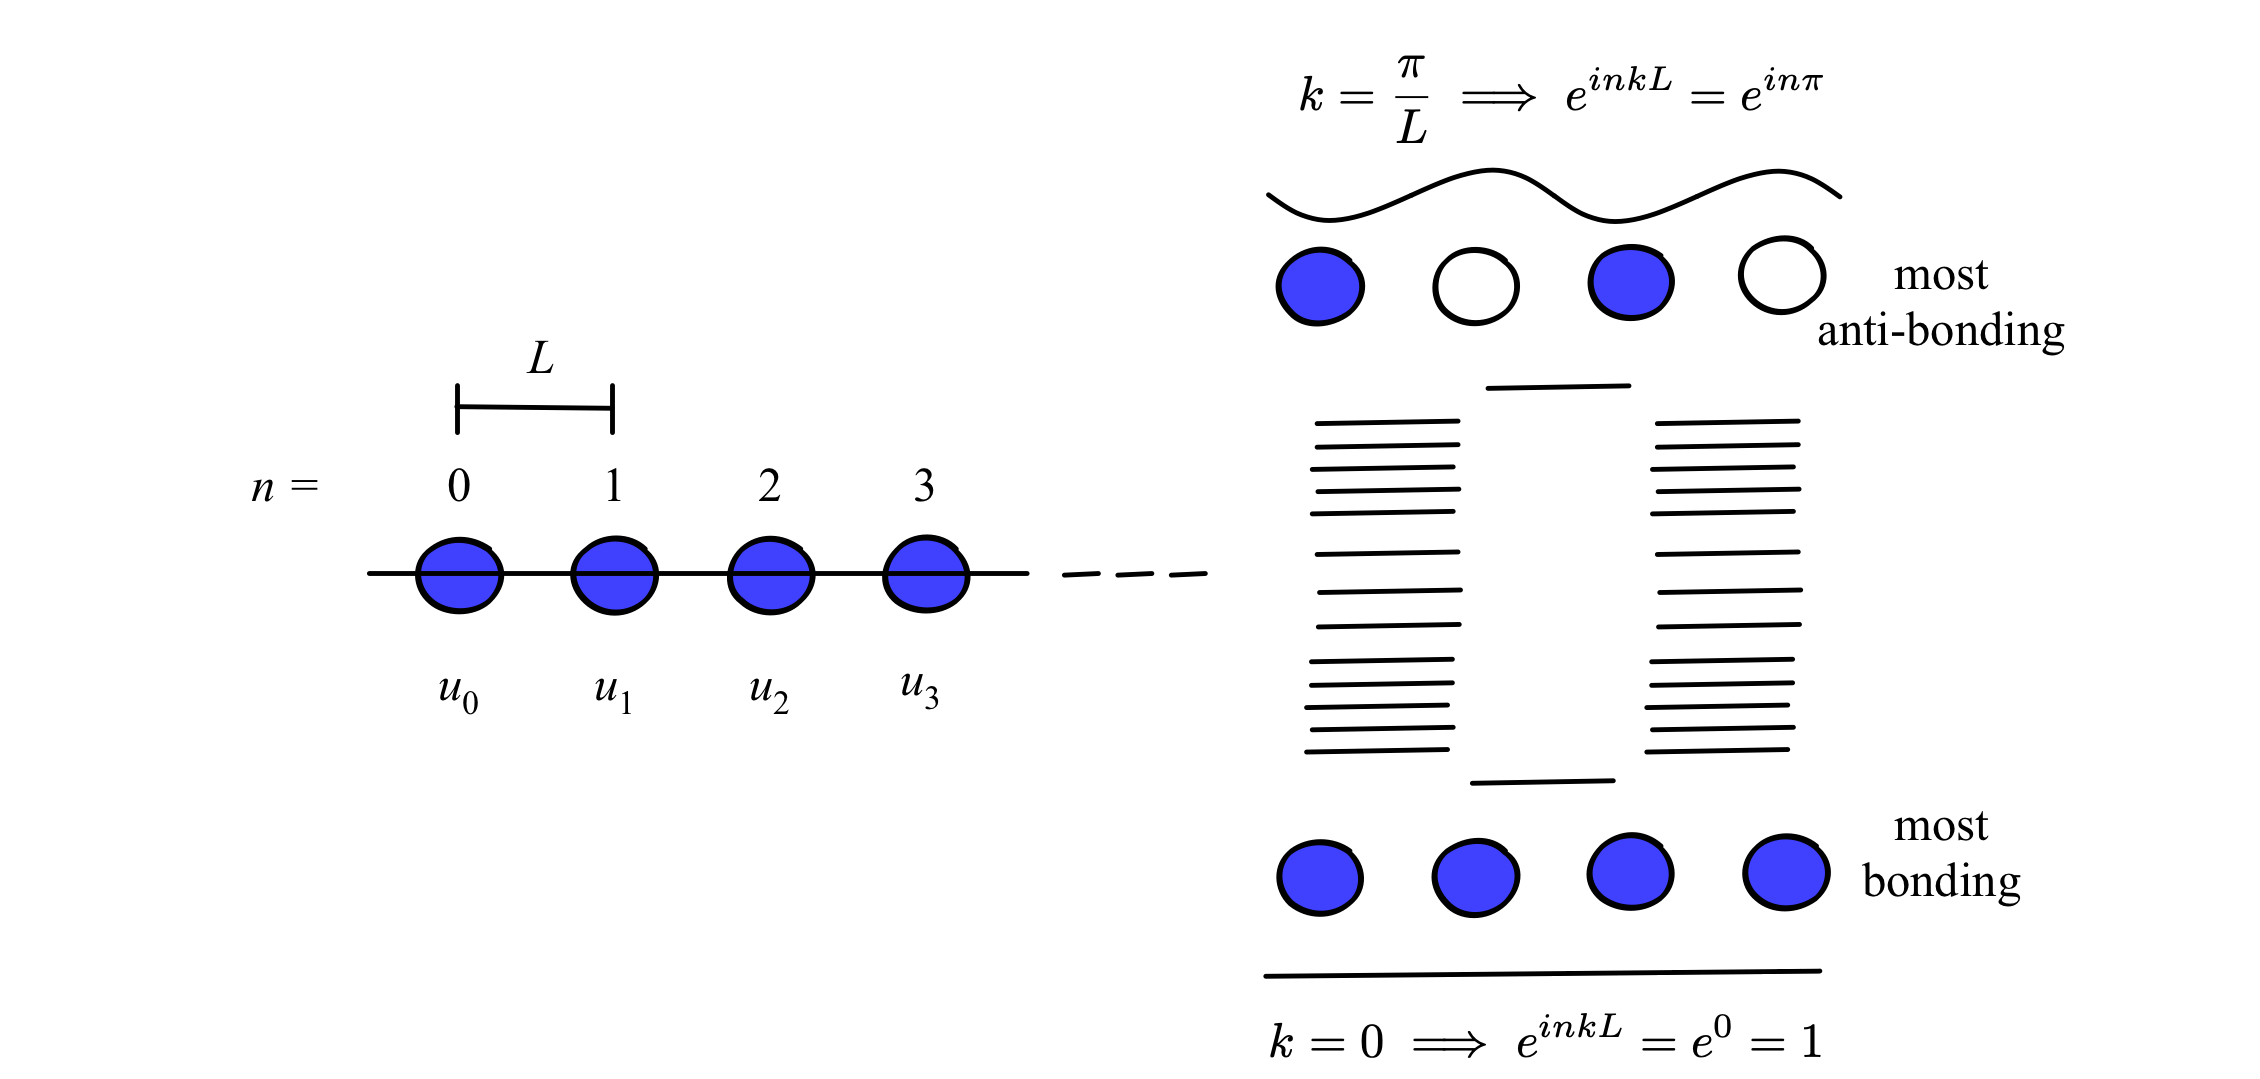
\includegraphics[width=1.0\columnwidth]{figures/ch3/bands.png}
  \caption[]{} 
  \label{bands}
\end{figure}

\subsubsection{Plane Wave Basis Sets}   %valence bands and conductions bands?

In the previous example the lattice periodic part of a bloch function took the form of a H 1s orbital. For more complex systems, $u_k(r)$ can itself be expanded into a plane wave basis set whose wave vectors $G$ are reciprocal lattice vectors

\begin{equation}
u_nk(r) = \sum_Gc_{n\textbf{k},\textbf{G}}e^{i\textbf{G}\cdot\textbf{r}}.
\end{equation}

The complete expanded Kohn-Sham wavefunction can be expressed as

\begin{equation} \label{KSeigenstates}
\psi_k(r) = \sum_Gc_{\textbf{k},\textbf{G}}e^{i\textbf{k+G}\cdot\textbf{r}}
\end{equation}

A plane wave basis set is often used for extended systems as they are inherently peroidic. The software used for the DFT calculations in this thesis, \ce{VASP}\autocite{}, uses a plane wave basis set. For DFT calculations applied to localised systems, such as molecules or nanoparticles, localised basis sets such as gaussian orbitals can be used. This is implements in software such as \autcite{}.

Sudden changes in electron density are hard to capture using a plane wave basis set (to take the extreme example, the fourier decomposition of a simple top hat in real space needs requires an infinite summation in reciprocal space). This can be problematic when describing the region around the nucleus where there are strong oscillations in the wavefunctions. However these oscillations are associated with the core electrons which are less important in chemical bonding, and so pseudopotentials - an effective potential without oscillations - can be used. It has been established that for certain systems pseudopotentials are as precise as all-electron calculations.\autocite{Lejaeghere2016a}
%http://helper.ipam.ucla.edu/publications/maws3/maws3_6085.pdf
%http://davidbowler.github.io/AtomisticSimulations//blog/dft-reliability#R3

\subsubsection{Optimising the atomic and electronic structure}

In this section the process of optimising the atomic and electronic structure of a system towards the ground-state (minimum energy) configuration is outlined. 

In Section \ref{DFTtheory} (Figure \ref{decouple}) we saw that the potential $v_\textrm{ee}$ is dependant on electron density $\rho$, which is itself dependant on $v_\textrm{ee
}$. Therefore an iterative method, the Self Consistent Field (SCF) method, is used to calculate the ground-state electronic structure (Figure \ref{SCF} in light blue). The initial guess for the density $n(r)$ is given by a superimposition of the atomic charge densities. This is used to calculate the potential and solve the KS equations, which gives a new $n(r)$. This process continues until the convergence criteria is met (most often within an energy tolerance). Various optimisation routines are provided in DFT codes for finding the ground state configuration, including the conjugate gradient scheme, Davidson Scheme and RMM-DIIS.

DFT is also used to find the ground state atomic structure. Structures from X-ray Diffraction Data are used as a starting guess, so that finding the energetic minimum becomes a local optimisation problem. Ions in the systems are displaced (either the internal coordinates of the unit cell or the unit cell parameters themselves are adjusted) and the electronic structure for that geometry is solved self-consistently. This repeats until the forces on each atom are zero (within a given tolerance, Figure \ref{SCF} in dark blue). 

\begin{figure}[h]
\centering
  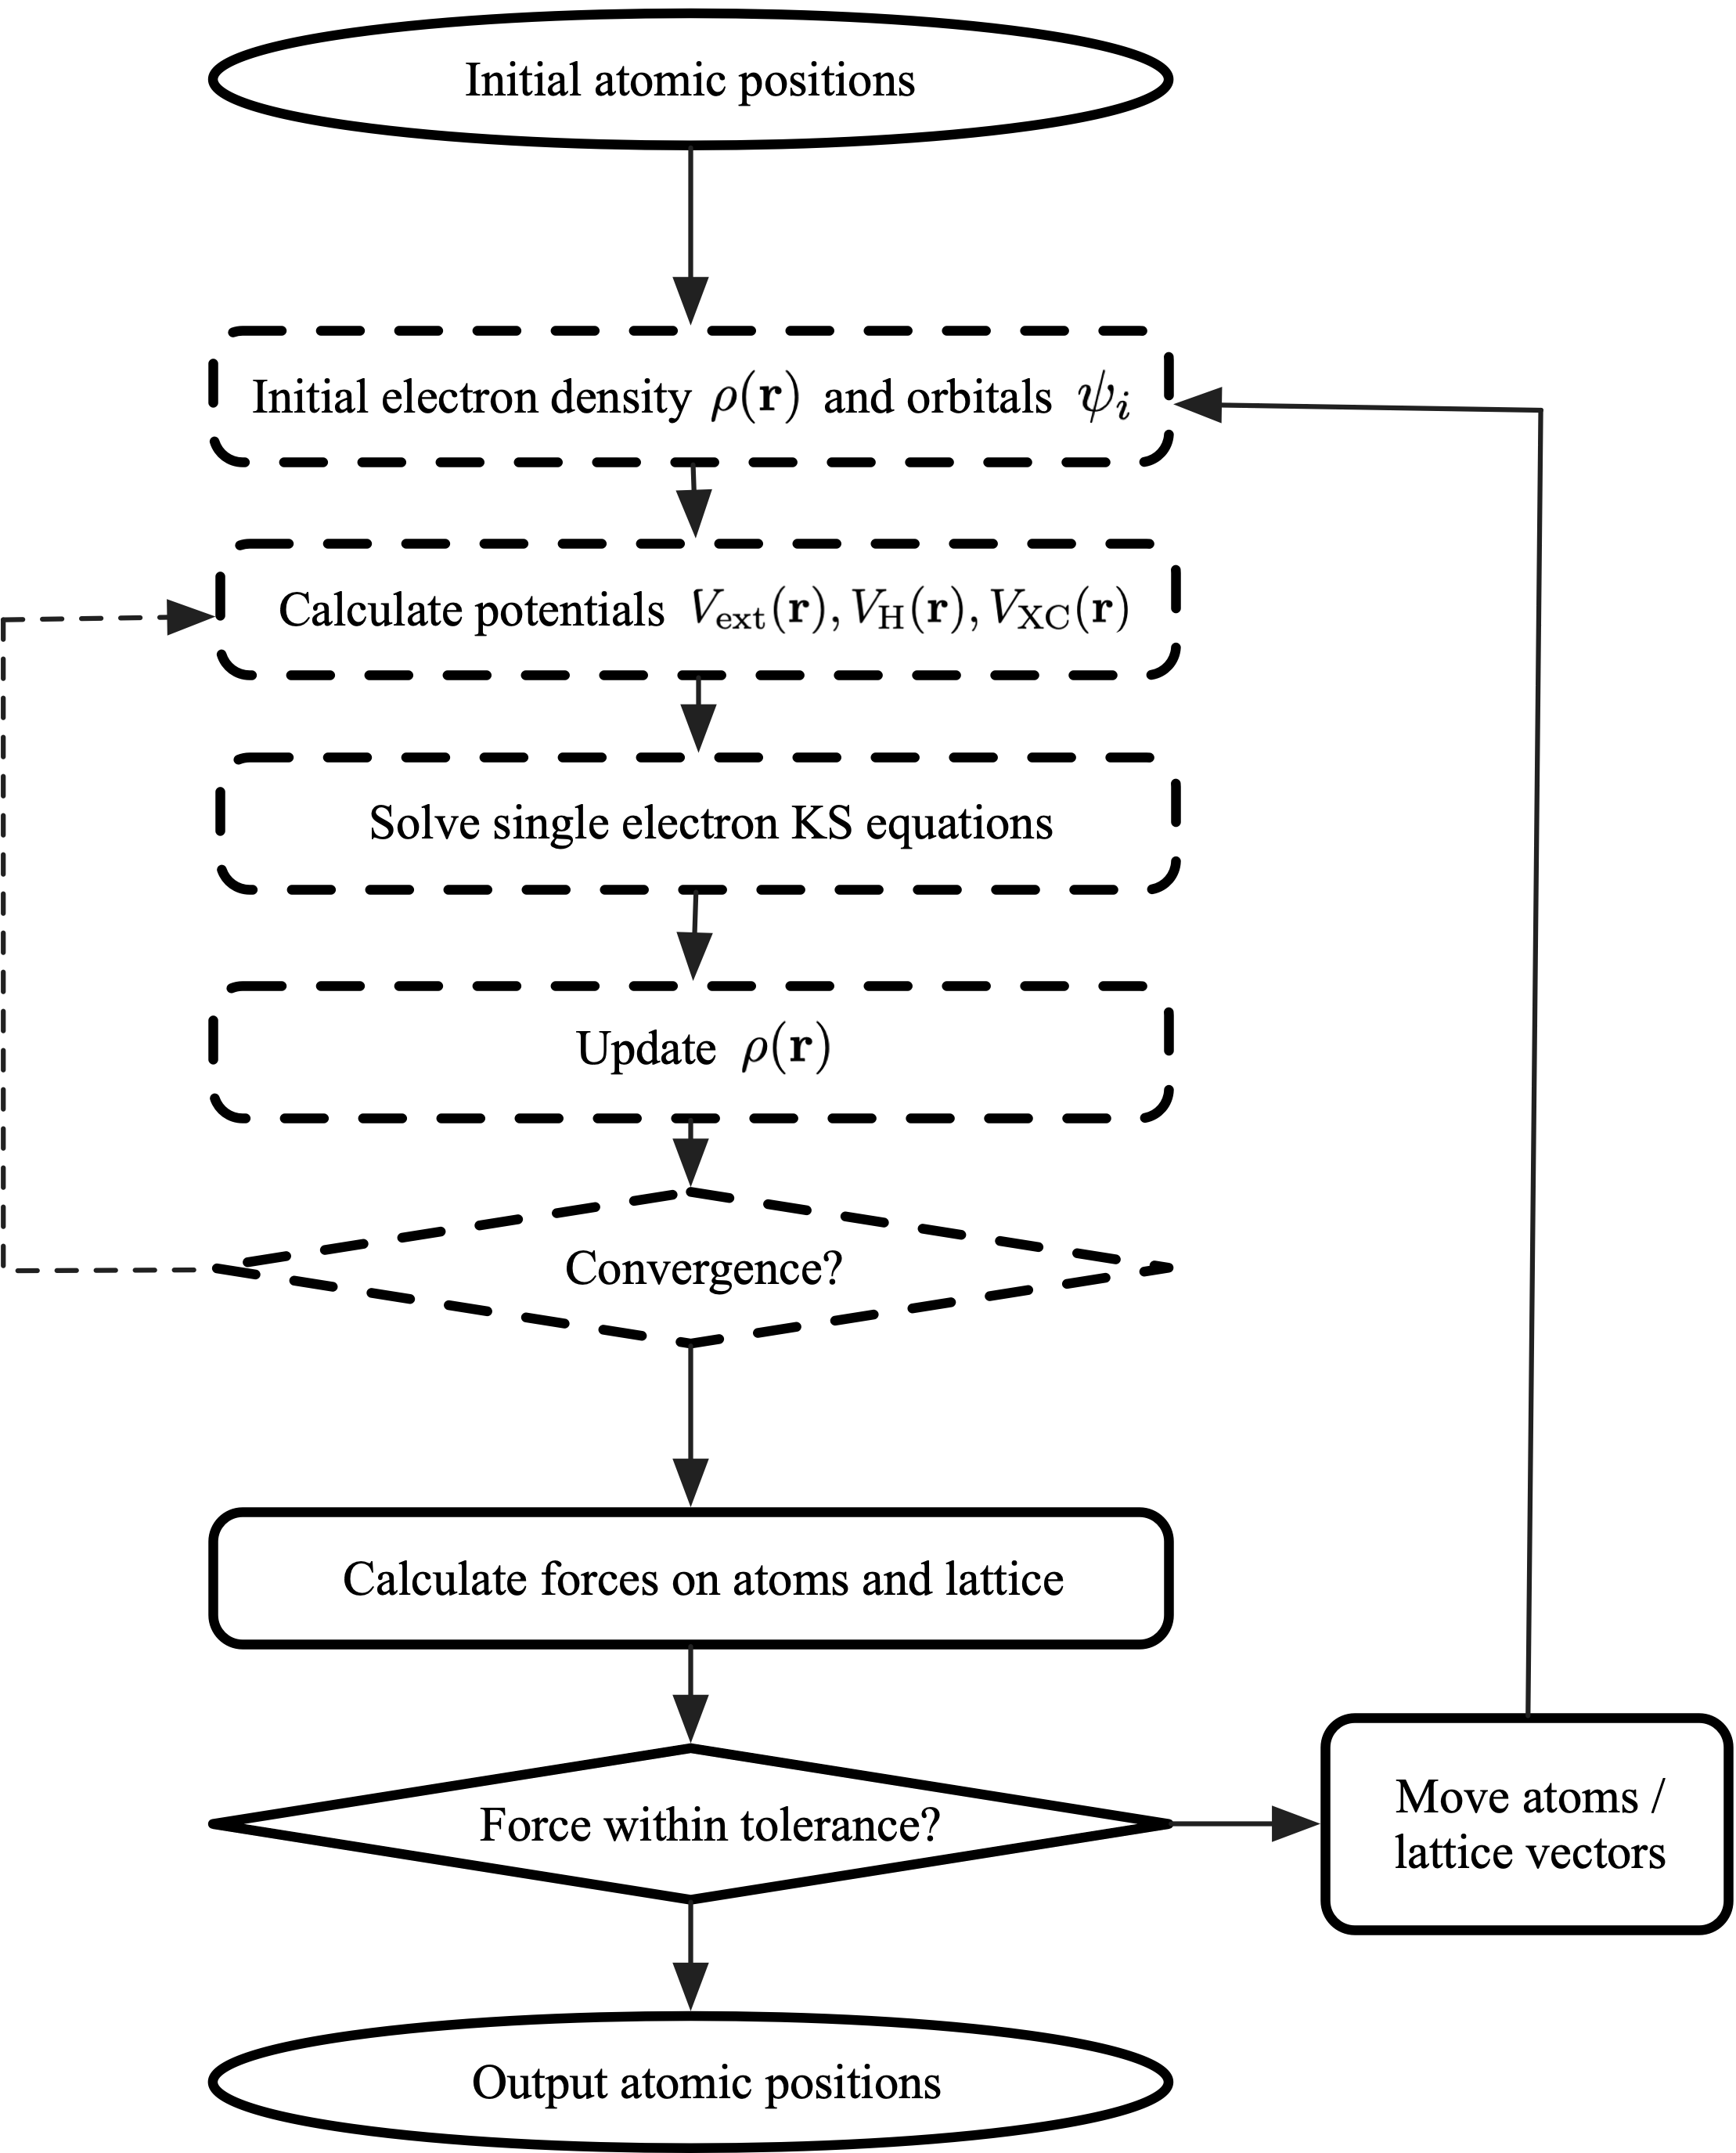
\includegraphics[width=1.0\columnwidth]{figures/ch3/scf.png}
  \caption[]{} 
  \label{SCF}
\end{figure}

\subsubsection{The limits of DFT}

\textit{Thoeretical limitations}

In Section \ref{DFTtheory} we outlined the approximations inherent to DFT calculations: the Born-Oppenheimer approximation and the unknown exchange-correlation functional. Higher levels of theory, which incorporate the effects of spin and relativity (e.g. spin-oribt coupling) are included in many DFT implementations. However DFT is still restricted to ground-state properties and higher levels of theory (GW or TDDFT) are required to describe optical excitations, for example. Another inherent limitation is that the KS eigenvalues are artificial; only the ground state electron density and derived properties are correct. In practice, the KS eigenvalues are used to calculate the band gap, although quantitative band gaps often require the use of hybrid functionals which are tuned to give the correct band gap.

\textit{Numerical limitations}

There is also a different set of approximations that relate to  numerical convergence rather than the underlying theory.

First, we have seen that the Kohn-sham wavefunctions are expanded in a basis set. In principle an infinite set may be needed to describe the Kohn-Sham wavefunction; in practice the basis set must be truncated. The kinetic energy operator is given by $-\frac{\hbar \Nabla^2}{2m}$. When this is applied to the plane wave Kohn-Sham eigenstates as given in Equation \ref{KSeigenstates}, we find that the kinetic energy is proportional to $|k+G|^2$; faster oscillations correspond to higher energy. A cutoff energy $\textrm{E}_\textrm{cut}$ is defined so that
\begin{equation}
\frac{1}{2}|k+G|^2 < \textrm{E}_\textrm{cut}.
\end{equation}
This cutoff energy must be tested to ensure that the property of interest, most often energy, is converged to within a certain range.

Second, to calculate many properties of interest we need to integrate over the Brillouin Zone. To calculate the total energy of an insulator for example, we use
\begin{equation} \label{energyintegral}
    E = \frac{\Omega}{(2\pi)^3}\sum_\textrm{occ.}\int_\textrm{BZ}E(\textbf{k})d^3k
\end{equation}
where $\Omega$ is the volume of the Brillouin zone and there is a sum over all occupied bands. 
In practice we do not know the continuous form for $E(\textbf{k})$ and so we evaluate Equation \ref{energyintegral} numerically as a weighted sum over special points in reciprocal space which form a $k$-point mesh. This is often an equally spaced mesh centred on the $\Gamma$-point ($k=(0,0,0)$) in reciprocal space (Figure \ref{MPgrid}). As with plane waves, there is a balance between accuracy (the higher the number of $k$-points, the higher the accuracy) and computational expense. This is demonstrated in Figure \ref{kpointconvergence} where x required a $k$-point grid of y to achieve convergence to within z.

\begin{figure}[h]
\centering
  \includegraphics[width=1.0\columnwidth]{figures/ch3/MPgrid.png}
  \caption[]{} 
  \label{mPgrid}
\end{figure}


\begin{figure}[h]
\centering
  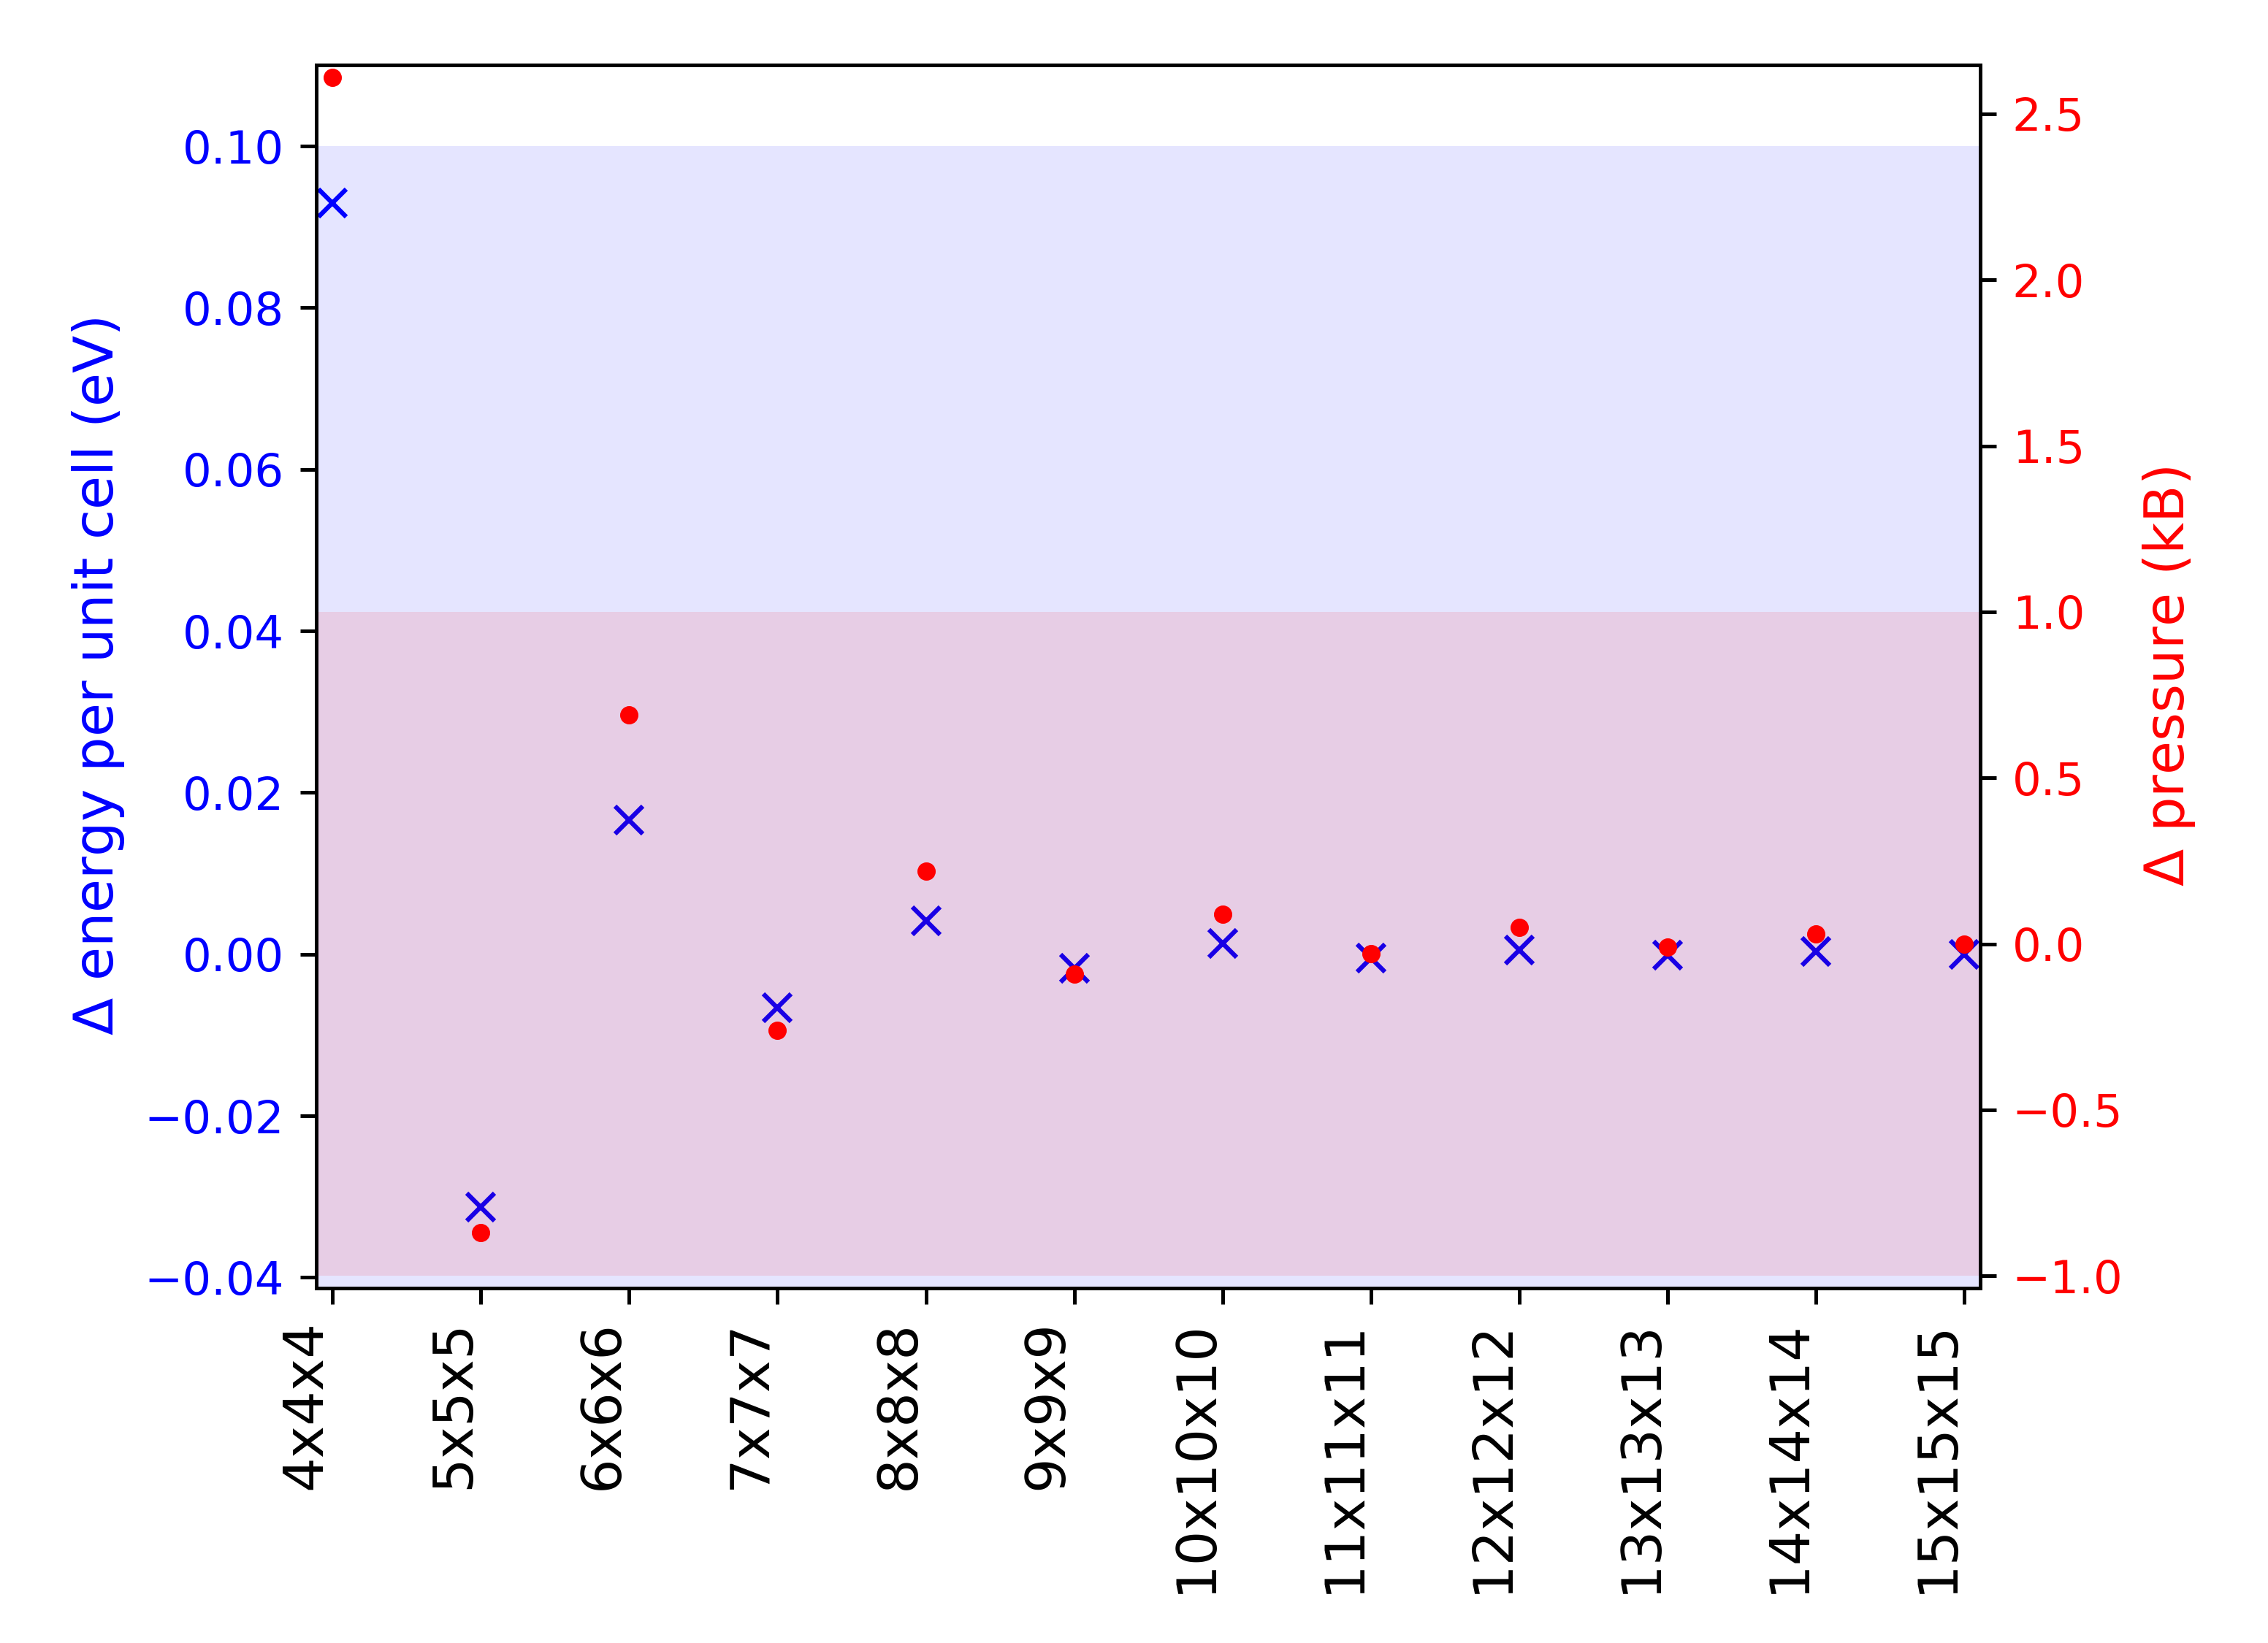
\includegraphics[width=1.0\columnwidth]{figures/ch3/kpointconvergence.png}
  \caption[]{} 
  \label{kpointconvergence}
\end{figure}

% - K-point grids and the commensurate grids for supercells.
% - Doubles k-points reuired as k and –k now no longer equivalent (SoC?)

%All convergence tests must be done for the property of interest. Cancellation of errors can mean that energy differences converge faster than ground state energies, as is reported in Chapter \ref{}.   % EP coupling calcas 

% include some convergence testing here.



% - See: Designing meaningful density functional theory calculation in materials science - a primer Anne E Mattson et al. Model. Sim. Mater. Sci Eng. 13 R1-R31 (2005). : for information about convergence and getting meaningful results.

%\textit{Computational limitations}
% - history of computers section at science museum for HPC section
% - put the amount of computer time and carbon burnt here?
% - computational expense: limitations on size: See review of materials models which Alison Walker mentions. Mesoscopic bridges the atomistic with the drift diffusion models. Meso is often monte carlo, tranjectory tpe calculations. Cells are too big for atomistic (1 cm squared). Efficiecny depends upon J-V curves which can only be modelled at scale of fill device. The electrostatics is incredible important which linked ot build up of charges at SC nd OC. Grain boundaries and recombination at intercaes.





\clearpage

\section{Calculating the properties of defects in semiconductors}

%% Books: 
% We are interested in calculating the electronic structure properties which lead to a description of the defects (trap density, binding energy, trap level, capture cross section).

%Mott and Littleton, 1938 - predict concentrations from the defect itself. And predict the conductivity.
% - THey are demainding and computational expensive .n To avoid computationally expensive defect calculations descriptors have been built on the idea of ‘defect tolerant’ materials: http://pubs.acs.org/doi/pdf/10.1021/acs.nanolett.5b04513

\subsection{Classifying defects}

% - many possible defects

% - many possible point defects

% - may be able to say defect is there experimentally but another step to identify which it is. Admittance spectroscopy, DLTS. 

% - defect levels deend on temperature. DLTS assumes T-independant scattering cross sction, not accurate,

\subsection{The energetics of defect formation}

% - calculating concentrations is difficult because it is exponentially sensitive to the formation energy. The other problem is that is dependant upon the chemical potential which is difficult to monito

% - History:

% - 1912 Born and Karman . PBC (first lattice dynamics paper)

% - 1925 Frenkel – formation of frenkel pair (first defects paper)

% - 1922 Jost – probability of forming defects. Tied into experimental work popular at the time, looking at how a material can be an ionic conductor when it is electrically insulating

% - 1938 Mott – the Mott-Littleton approach for calculating defects

% - defect energies theoretical founsations - mott littleton (1938)  - a way to calculate E the defecct energy as knew the hopping rate expression, but didnt know E. only experimental input is dielectric constant.see special 1988 issue.

% - Fermi level pinning (?) / defect concentration: Happens in TCO’s such as FTO. Above a certain concentration there are no more holes. This could happen when there are defect complexes which compensate each other.

% - This is a compensation mechanism. We try to adjust the fermi level of the system by introducing impurities. However above/below a certain energy level there is spontaneous formation of defects (defects which have a negative energy of formation). These defects compensate for the impurity and in this way the fermi level is pinned.


% - There is a linear dependance on the product of charge and fermi energy. This means that the slope of the formation energy when plotted against fermi energy gives the charge state. It also means that neutral charge states are flat

% - Calculable and observable table:
% Delta E : heat of formation / concentrations
% Defect ionisation – optical – instanataneour: PL, optical absorption / photoconductivity
% Defect ionisation , thermal, after relaxation: DLTS / thermally stimuated conductuvtiy
% Defect vibrational modes: IR/raman spectra and recombination rates

% - Defect levels are very sensitive to the level of theory used (see schematic under visuals) - important to use correct one.

\subsection{The supercell method}

% - Finite size effects (supercell)

% - Other method - embedding. 

% - The supercell method leads to some unphysical results for both electronic and vibrational properties. The defect will perturb the lattice. The SC method captures localised defect effects well – but the delocalised defects (possibly in the band) are not captured as there is an enforced periodicity. The only way around this is to use greens functions method (phonons) or QM/MM approach (electrons).


\subsubsection{Supercell corrections}


% - Leslie nad Gillan - charged defects in supercells first paper. their correction gives a size dependance on the size of supercell (it is a monopole expansion and known as Markov Payne correction).

%-one charge correction is the process of getting a meaningful fermi energy (shift in potential energy -core level shift)
%-coulomb charge correction: MP correction or LZ (which accounts for Moss Burstein filling)

% - for a really good explanation see Suzys group talk (Monday the 10th september 2018) and https://aip.scitation.org/doi/10.1063/1.5029818 which it was based upon.

% Spurious charge nteractions as a sresult of the SC approach. For example, 1. periodic-periodic defect-defect interaction and 2. defect-background charge interactions.
% - Leslie Giliian point charge correction
% - MP point charge but the defect charge distribtiion is ill defined.
% - FNV point charge correction indirectly calculates the MP. Pascalrello
% - Oba correction.

\section{Calculating the properties of vibrations in crystals} \label{sec:latticedynamics}
%% Hellmann Feynmann theorem

%%: Books

% - Stationary atoms would conflict with the H.U.P which tells use that we cannot know the both the position and momentum of a particle exactly. At T=0 there is zero point motion.  Evidence for this in the zero point motion renormalization. 

% - As temperature increases the motion increases in amplitude with thermal energy. We know this affects electrical and optical properties – look at the peak shift in energy and peak broadening ith temperature.

% - For small amplitudes we consider a simple harmonic motion.

% - At larger amplitudes we must consider anharmonic motion.

% - The motions are determined by atomic forces. For a 1D system with a single mass or with two masses (lattice with basis) we can solve analytically. Otherwise these can be determined through DFT calculations, producing a force constant matrix. 

% - Acoustic  waves, or sound waves. For each frequency and direction there are three waves each with different polarization (one longitudinal, two transverse)

% - Acoustic waves are called acoustic as they approach speed of sound (linear dispersion) at long wavelength (small k). Optical are called optical as as k tends to 0 there is coupling with electromagnetic waves.
% In 3D crystal with one atom per unit cell there are 3N modes (N unit cells). N modes per lattice branch. Two transverse one longitudinal.
% In 3D crystal with two atoms per unit cell there are 2 x 3N modes (acoustic and optical).


% - Uncoupled oscillations = normal modes. Each k has a definite w and oscillates independantly of other modes.

% - Adding 2pi/a to k does not alter the atomic displacements or group velocity: it does not affect any physical observable of the system. Can consider all possibilities in a 2pi/a region.

% - At pi/a there is bragg reflection (simply take braggs law). These create standing waves: the wave is dispersionless (no velocity! Standing!)
% In long wavelength limit the waves are disperionlessness.

% - For two types of atom: There are two roots to the equation connecting w and k.
% No matter how many atoms there is still periodicity of 2pi/a.
% There are now 2N normal modes. (N number of unit cell). A is unit cell length.

% - model for vibrations (harmonic approximation) ---> vib freq and displacement patterns (vibrational spectra) and from that IR/raman, free energies (T) - phase change. all stuff you couldnt get with standard electronic structure

% - Partition function ---> bridge function kTlnZ (bridges micro and macro thermodyamics) to get helmholtz free energy. need vibrations to get temperature dependant energy and stability as a function of temperature.

% - Table with the approximation and the properties you can get....

% - Start with the full Xtal hamiltonian  adiabatic approximation to account for ifferent time scales  Taylor expansion  we are now viewing the chemical bonds as springs with a particular force constant.  (nice point for a sketch)

% - Other interactions could be accounted fotr at this point. For example, there could be a magnetic interaction expanded in terms of spins. Heisenberg interaction would ensure that J is diagonal. Force constant woulc be renormalised by these magnetic interactions

% - There are a multitude of ways to calculate these force constants: explicitly (finite difference, DFPT for 3rd or 4th orders), empirical potentials (TDEP), compressive sensing lattice dynamics or beyond perturbation (AIMD,PIMD,SCAILD, variational methodslike SSCHA developed by Ion Errea).

% - See Schematic idea for perturbative and non-perturbative regime.

% - Basically see p. 62 of stonehams defect and defect Processes in non-metallic solids for a great lo-down (molecules section!)

% - Adiabatic approximation: Can thin of electronic wavefunction for eignstate of nuclei fixed in position.

% - So far this has been fully classical. To make quantum we expect lattice vibration of frequency will be like simple harmonic oscillator and so will be restricted to certain energy values En=(n+1/2)hbaromega.
% The phonons of energy hbar omega have exact energy so cannot be localised in space: formed of delocalised plane waves
% But can construct localized packet using modes of different fequency. Can then treat phonons as localised particles. E = hbar omega. K is the crystal momentum .
% Phonons are bosons, not conserved. They can be created and destroyed. 

% - There are 3 major assumptions underlying standard phonon theory: 1) hat the equilibrium positions in a crystal are the minima of the born-oppenheimer potenetial energy surface where electron and nuclear motion are decoupled. May not be same as average position form the full electron-nuclear wavefunction . This is the adiabatic approximation. 2) harmonic approximation (cubed terms higher are ignored) 3) dipole approximation : higher multipole expansion are ignored

% - What information can we get from phonons? 
% Thermodynamic quantities at low temperature: heat capacity, entropy, free energy, zero-point,
% Phase transitions from the Gibbs free energy,
% Conductivity,
% Infromation about lattice instabilities in the form of imaginary frequencies,
% Elastic tensor from the q to zero limit of phonon dispersion,
% Thermal expansion coefficient,
% Temperature dependence of the band gap,
% Electron phonon coupling,
% Static polarization

% - Experimental evidence:
% Measured directly with inelastic scattering,
% IR and Raman spectroscopy

% - Extent of Anharmonicity depends upon how much of the potential energy space you are exploring ((tie in with perturbative and non-perturbative regime skethc). At low T you may be exploring harmonic potentil like minima, at High T you may be beyond this minima


\subsection{The harmonic approximation}

% - a potential energy surface and a bit highlighted with harmonic section (see schematics under visuals)

% - Taylor expansion of the crystal potential.

% - harmonic: truncate at second. potential energy is quadratic ---> linear restoring force. Near Q=0 they are good enough.

% - harmonic approximation expects the energy to increase as you push along the mode.imaginary frequency because $w^2$ is negative.
% dynamic stablity if all positive

% - quasi-harmonic:properties as a function of volume.helmholtz as function of temeparture  - at some point it is favourable to have a different volume . Free energy as function volume for several tempatures and the fit an equation of state. 

% - Then you can get the bulk modulus, heat capacity constant pressure, gibbs free, gruneisan, volumetric thermal expansion.use to get properties at finite T - use the structure which minimises for a particular temp.

% - Thermal expansion coefficients, system anharmonicity (e.g. modal grun parameters) and the temperature-dependence of other properties can be calculated in the quasi-harmonic approximation (QHA). 
% Here the lattice dynamics is harmonic at a given temperature; however, the cell volume is scaled by thermal expansion to give the first-order contribution of finite temperature effects. 

\subsection{Anharmonicity}

% - anharmonicity schematic under visuals: Si, PbTe, SrTiO3

% - anharmonicity double well schematic for perovskites, compared to single well schematic, and with posiion of electron indicated and renormalisation that can be used above the curie temperature (see schematic under visuals).

% - Double hat in SnSe and its seen in lots of things incl. octahedral rotations.

% - for patching you have to get the dynamical matrix for the soft mode calcultions, then manually change the entres for the renoarmlaised freucies, then work backards to get the force constant matrix, then re-generate the dynamical matrix and diagonalise.

% - harmonic freq that reproduces the anharmonic partition funciton.

% - All the macro thermodynamic observables have to go via the partition function anyhow.

% - Jacobs ladder of anharmonicity: harmonic/quasi-harmonic/anharmonic (3) / anharmonic Q4. The higher up you go,the more you can calculate.
% 2: freq an eigenvectors / helmohltz free energy (constant volume)
% spectral instensities
% quasi 2: gibbs free, soft mode, finite T structure/prop
% 3: phonon linewidths / spectral lifetimes
% 4: anharmonic frequency shifts

% - anharmonicity and thermal conductivity

% - The thermal conductivity as calculated in phono3py depends upon the single mode relaxation time approximation (see togo’s theory paper on this). This is where the lifetime as of a single mode as calculated in phono3py is set as the relaxation time in the linearised boltzmann transport equation.
% Under this assumption the thermal conductivity is then a summation over the product of heat capacity, mode velocity and relaxation time, which all come out of phono3py

% - see Aron blog post on anharmonicity.

% - harmonic approximation: lifetimes are infinite. Not true for processes involved with carrier capture, recombination and heat propagation.

% - Anharmonicity most important when under high pressure or high temperature (bouchert) which is often the case for geophysical applications.

% - To gauge anharmonicity can consider the 3-phonon scattering phase space: the phase space can be decreased with : large gap between acoustic and optical, isotopic pure heavy atoms, weak polarity, bunching of acoustic phonons….(Broido work)

% - Navaneeth : assessing how higher order anharmonicity can aggect htermal conductivity. In Diamond the 4 phonon phase space is 10x that of 3-phonon. In Bas it is 100X that of 3-phonon phase space. We must then also consider the scattering strength (can only consider the scattering rate of those with a large phase space). The size of these phase spaces are huge. For example, Bas which is in the zincbelnde structure has 6 polarisations. If each done explicitly there would be $9x10^ 3$-phonon calculations, for 4-phonon processes there would be $2x10^12$!!!  So instead temperature-dependent ensembles are used (where all atoms are moved at the same time, calculated from explicit 2nd order force constant calculation) and then used to fit 3rd and 4th order force constants to.

% - We can’t use DFPT when the perturbation is not small and there is strong, anharmonic behaviour. Use Ab-initio MD to capture this such asm the Green-Kubo method (fluctuation-dissipation theory) which relies upon the fact that thermal conductivity can be inferred from heat flux. [Heat flux is calculated from the stress tensor.] This gives a result which is anharmonic to all orders. The only restraint is that the system is in thermal equilibrium (linear response). Highly anharmonic motion is found in ZrO2, where there is very fast switching: like that seen in MAPI: severe violation of the harmonic principle, as seen in MAPI.

% - Phonons from DFPT: http://journals.aps.org/rmp/pdf/10.1103/RevModPhys.73.515 - a good outline of the theory implemented in phono3py.

\subsection{The finite displacement method}
.
% - Note that the  eigenvalue equation for the dynamical matrix is gotten from fourier transform
% Of the taylor expansion of the crystal potential. For derivatives we exploit the hellman-feynam theorem and use finite differences (the alternative would be the DFPT / linear response (which is first order DFPT))

% - See Jonathans talks

% - force constant matrix . then construct dynamical matrix - -> wavevector. then diagonalise - the eigenvectors and eigenvalues. do a schematic for this process. then two ways to get to the dynamical matrix.

% - Force constant via finite displacement - displace small and calculate force. Simple, general and can split into small jobs (parallelise). but need supercells. Maximum is 6N displacements but this is seriously reduced by symmetry.

% - perturbation theory- dynamical matrix directly. no supercell and more accurate but constrained which functionals and pseudopotentials you need.

% - Need good relaxation: don't skimp on the forces, cutoff or k-points.

% - Once the dynamical matrix is built, the rest is post-processing.

% - phonons can have a wavelength longer than the size of the supercell - need to capture the longer wavelength.

% - PBEsol for reproducing lattice constants and phonons (Jonathan 2015 J.Chem. Phys)

\section{Summary}




